\section{Versuchsdurchführung}

\subsection{Bestimmung der Relaxationslänge}

Um die Relaxationslänge $\lambda$ schneller Neutronen in Wasser zu messen, wird die Anzahl der Neutronen pro Zeiteinheit in Abhängigkeit des Abstandes von der Quelle gemessen. Es wird im Bereich $14$ bis $\SI{19}{\centi\metre}$ gemessen.
Da der Neutronenfluss proportional zur Anzahl der Neutronen ist, und da die anderen relevanten Größen (Zeitintervall und Detektorfläche) nicht variiert werden, kann daraus die Relaxationslänge bestimmt werden. Durch Logarithmieren des Flussgesetzes ergibt sich
\begin{equation}
 \ln\left(Nr^{2}\right) = -\frac{r}{\lambda} + C,
\end{equation}
mit der Anzahl der Neutronen $N$, der Distanz zur Quelle $r$ und einer Konstanten $C$. Durch eine lineare Regression kann nun $\lambda$ bestimmt werden.

Die Vorraussetzungen, damit dieses Flussgesetz gilt, sind jedoch im Experiment nicht erfüllt. Das $^{10}$B-Zählrohr kann nur Neutronen bis zu einer Energie von ca. $\SI{100}{\kilo\electronvolt}$ detektieren. Somit werden gerade die schnellen Neutronen nicht gemessen. Dennoch folgt die folgt die Verteilung der Neutronen im Experiment dem obigen Zusammenhang.
Der Grund dafür ist, dass die langsamen Neutronen sehr stark an den Protonen des Wassers gestreut werden. Dabei verlieren sie einen Großteil ihrer Energie. Daher entfernen sie sich nur bis ca. $\SI{3}{\centi\metre}$ von der Quelle. 
Der gemessene Fluss verhält sich daher für Abstände $>>\SI{3}{\centi\metre}$ wie der Fluss schneller Neutronen.

\subsection{Bestimmung der Diffusionslänge}

Um die Diffusionslänge $L$ thermischer Neutronen in Wasser zu messen, kann nicht auf analoge Weise zum vorherigen Versuch vorgegangen werden, da es keine Punktförmige Quelle thermischer Neutronen gibt.
Stattdessen wird die sogenannte Cd-Differenzmethode verwendet. Dazu wird die Quelle mit Hilfe einer dünnen Cadmium Kugelschale abgeschirmt. Der Absorptionsquerschnitt für Neutronen in Cadmium (s. Abb. \ref{fig:cd}) ist für thermische Neutronen deutlich größer als in den anderen Energiebereichen. Daher durchqueren nur schnelle Neutronen die Kugelschale.
Durch Differenzbildung mit dem gesamten Fluss erhält man den Fluss einer thermischen Neutronenquelle. Die Diffusionslänge kann nun durch eine lineare Regression der Form
\begin{equation}
 \ln\left(N_{d}r\right) = -\frac{r}{L} + C,
\end{equation}
mit der Differenz der Neutronenzahlen $N_{d}$, bestimmt werden.

\begin{figure}[tb]
  \centering
  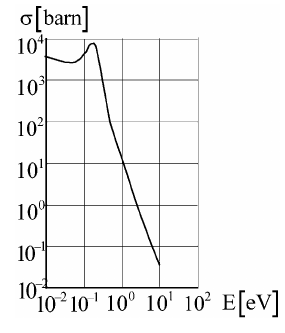
\includegraphics[scale=1.0]{./fig/cd_wirkungsquerschnitt.png}
  \caption{Absorptionsquerschnitt für Neutronen in Cadmium \cite{BB}}
  \label{fig:cd}
\end{figure}